\subsection{Lecture 20}
\subsubsection{Vertex Cover, Clique}

We now consider the Vertex Cover problem. First we define what a vertex cover is.

\begin{definition}[Vertex Cover]
    A vertex cover is a subset of vertices $S \subseteq V$ where $\forall e \in E$, $\exists v \in S$ such that $e$ has $v$ as
    one of its endpoints.
\end{definition}

Now, the Boolean Vertex Cover problem is focused on:
\[ \textsc{VertexCover} = \{\langle G, k\rangle : \exists \text{ vertex cover of $G$ of size $\leq k$} \]

The reduction then follows from the following claim:
\begin{theorem}
    $S$ is a vertex cover if and only if $V \setminus S$ is an Independent set.
    \begin{proof*}
        First, assume $S$ is a vertex cover. Suppose $V \setminus S$ was not an independent set. This would mean two
        vertices $a, b \in V \setminus S$ are neighbors. However, this would mean that $(a, b)$ is not covered by $S$, which is a contradiction,
        since $S$ is a vertex cover. Thus, by contradiction, $V \setminus S$ must be an independent set.

        The other direction is similar.
    \end{proof*}
\end{theorem}

This means that the reduction can be summarized as the following. Given an input $\langle G, k \rangle$ to independent, we will reduce to vertex cover
with input $\langle G, n - k \rangle$. This will find if there exists a vertex cover of size $\leq n - k$, which if there is, can be converted
to an independent of size $\geq n - (n - k) = k$. Thus, the reduction was successful.

Now, we consider the clique problem.

\begin{definition}[Clique]
    A clique is a set of vertices that have all possible edges between them in the graph.
\end{definition}

Now, the Boolean Clique problem asks:
\[ \textsc{CLIQUE} = \{ \langle G, k \rangle : G \text{ has a clique of size $\geq k$} \]

One can make a similar observation. Note that any independent set in $G$ is the same as any clique in the complementary graph (i.e. with the edges
not present added and the ones not present removed).

\subsubsection{3D Matching}

We now look at a generalization of max bipartite matching. In 3D matching, we use triples. Given $n$ boxes, cars, and drivers,
\[ b_1, \dots, b_n, c_1, \dots, c_n, d_1, \dots, d_n \]
Let $T = B \times C \times D$. The 3D Matching problem asks, does there exist a subset of $T$ which covers each box, car, and driver exactly once.

Consider a special case of 3SAT.
Consider some instance $\phi$. It is true if $\phi$ is satisfiable 3SAT instance, and each literal in $\phi$ occurs $\leq 2$ times.
We will show 3SAT reduces to this (3SATL2) and then we reduce to 3D matching.
\begin{algothm}[Reduction 3SAT to 3SATL2]
    Say $\phi$ is a 3SAT instance on $n$ variables $x_1, \dots, x_n$.
    First, we can simplify $\phi$ by removing any variable $x_1, \dots, x_n$ that only appears positive or negative. 
    Suppose some literal $x$ that appears $t > 2$ times (positive or negative). Then, we create $t$ new variables $y_1, \dots y_t$ and replace the $i$th occurrence
    of $x$ with $y_i$. Now, to enforce these variables to be equal, we just add the clauses:
    \[ (y_1 \lor \overline{y}_2) \land (y_2 \lor \overline{y}_3) \land \dots \land (x_n \lor \overline{x}_1) \]
    Note that now, each of the $y_i$ appears at most twice (counting positive and negative separately), so we have reduced to an equisatisfiable form.
\end{algothm}

Now, we show the 3SATL2 $\to$ 3DM.
\begin{algothm}
    Given $\phi$ on variables $x_1, \dots, x_n$ with clauses $R_1, \dots, R_m$. For each $x_i$, draw the following diagram.

    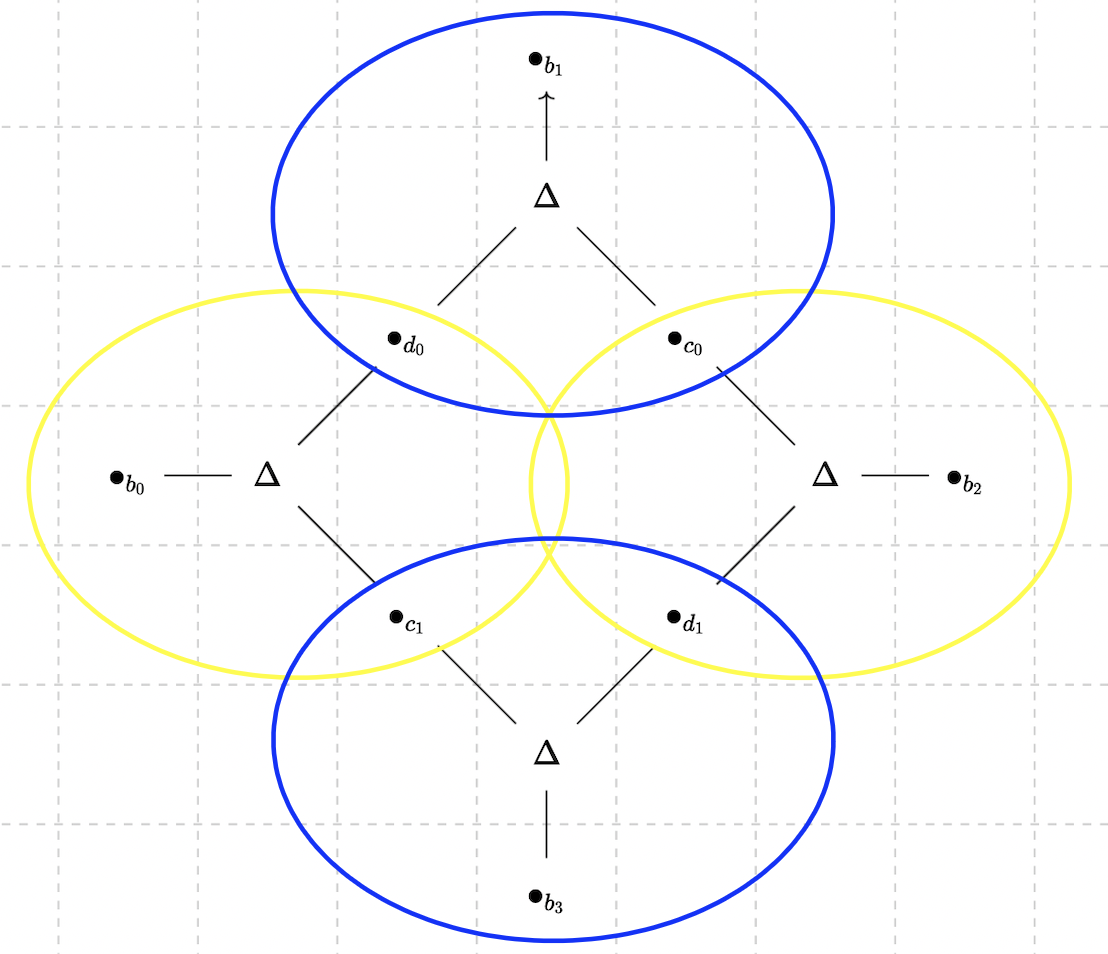
\includegraphics[width=100mm]{gadget3dm.png}

    Each triangle is a triple and each dot is a box, car, or driver. If we want to cover all cars and drivers, must either take blue triples (call this $x_i = False$)
    or yellow triples (call this $x_i = True$). Now, repeat that "picture" $n$ times. Furthermore, we need to add more boxes, cars, drivers, and triples
    to ensure that the clauses are also followed. Consider some clause $R$, for example,
    \[ R = (x \lor \overline{y} \lor z) \]
    Then, we introduce a new car $c_R$, driver $d_R$, and 3 new triples (one per literal in the clause). For our example we use:
    \begin{itemize}
        \item $x$ - add triple $(b_{x_0}, c_R, d_R)$ or $b_{x_2}, c_R, d_R)$
        \item $\overline{y}$ - add triple $(b_{y_1}, c_R, d_R)$ or $(b_{\overline{y}_3}, c_R, d_R)$
        \item $z$ - add triple $(b_{z_0}, c_R, d_R)$ or $(b_{z_2}, c_R, d_R)$
    \end{itemize}
    this is why we said we needed 3SATL2, because our diagram can only suppose 4 boxes per variable (each variable can only participate in 2 clauses
    positively and 2 negatively). However, you might have some leftover boxes,
    if each variable participates in less than 2 clauses. Note that there are $4n$ boxes introduced (from the diagrams), and we matched $2n + m$ of the cars/drivers.
    Thus, there are $4n - (2n + m) = B$ boxes left.
    Thus, we can introduce $B$ new cars and drivers who are willing to take any box. We then match the last $B$ boxes with these "dummy" cars. Now, we have turned our
    3SATL2 instance into a 3DM instance on $4n$ cars, boxes, and drivers. Thus, we have completed an efficient reduction.
\end{algothm}

\subsubsection{ZOE, Integral LP}
We now turn to the problem of systems of zero-one equations. We are given $A \in \{0, 1\}^{m \times n}$. The ZOE problem asks if there exists
$x \in \{0, 1\}^n$ such that $Ax = \textbf{1}$.

We state that there is a reduction from 3DM to ZOE.
\begin{algothm}
    Take our instance $b_1, \dots, b_n, c_1, \dots, c_n, d_1, \dots, d_n$ where there are $m$ triples among the items (3-cliques). Define
    \[ A_{ij} = \begin{cases}
        1 & \text{if $i$ row participates in $j$th triple} \\
        0 & \text{otherwise}
    \end{cases}\]
    Note that $A \in \{0,1\}^{3n \times m}$. Then, finding a solution to this ZOE instance leads to what follows. Consider some box $b$ which is at row $i$. After doing the matrix multiplication,
    we have $\sum_{T \in \{\text{triples containing b}\}} x_T = 1$, i.e. exactly one of these triples must exist. This is exactly what 3DM wants, so solving the ZOE instance
    finds us a matching such that exactly one triple exists for each item.
\end{algothm}

Now, we discuss integral linear programming, which is linear programming with added integrality constraints (require some variables to be integers).
The decision problem writes:
\begin{align*}
    \exists x? c^T &\geq k \\
    Ax &\leq b \\
    \forall i \in S, &x_i \in \mathbb{Z}
\end{align*}

Reducing ZOE to Integer LP is not too hard. We make an Integer LP with the following objective and constraints.
\begin{itemize}
    \item $k = -\infty$ (we only care about feasibility)
    \item Constraints: $Ax = \textbf{1}$
    \item $\forall i, 0 \leq x_i \leq 1$
    \item $S$ is the set of all variables.
\end{itemize}